\documentclass[11pt, a4paper]{article}

% Packages
\usepackage[francais]{babel}
\usepackage[T1]{fontenc}
\usepackage[utf8]{inputenc}

\usepackage[left=2cm, right=2cm, top=2cm, bottom=2cm]{geometry}
\usepackage{fancyhdr}
\usepackage{lastpage}
\usepackage{hyperref}
\usepackage{float}
\usepackage{graphicx}
\graphicspath{{./img/}}

% Reset paragraph indentation -------------------------------------------------
\setlength{\parindent}{0cm}

% Page header and footer ------------------------------------------------------
\pagestyle{fancy}
\setlength{\headheight}{14pt}
\renewcommand{\headrulewidth}{0.5pt}
\lhead{Algorithmes avancés}
%\lhead{\includegraphics[height=1cm]{logo.jpg}} % Change \headheight to right size
\chead{Clustering et classification supervisée}
\rhead{Claudio Sousa, David Gonzalez}
\renewcommand{\footrulewidth}{0.5pt}
\lfoot{10/06/2018}
\cfoot{}
\rfoot{Page \thepage /\pageref{LastPage}}

% Table of contents depth -----------------------------------------------------
\setcounter{tocdepth}{3}

% Document --------------------------------------------------------------------
\begin{document}

\title
{
    \Huge{Algorithmes avancés} \\
    \Huge{Clustering et classification supervisée}
}
\author
{
    \LARGE{Claudio Sousa, David Gonzalez}
}
\date{10/06/2018}
\maketitle

\thispagestyle{empty}

%\tableofcontents

\newpage

% -----------------------------------------------------------------------------
\section{Introduction}

Le but de ce travail pratique pour le cours d'algorithmes avancés est de mettre en pratique
les différentes techniques en science des données,
plus particulièrement, le clustering ainsi que la classification des données. \\

Ce travail est divisé en 3 parties:
\begin{itemize}
    \item clustering de données imposées;
    \item classification supervisée avec algorithmes d'apprentissage et données imposés;
    \item classification supervisée avec algorithmes d'apprentissage et données libres.
\end{itemize}

\subsection{Normalisation des données}

Les données utilisées durant ce travail pratique peuvent être de différentes natures et
requièrent d'être normalisées.

En effet, certaines méthodes qui sont utilisées pour ce travail souffrent beaucoup des facteurs d'échelle,
ce qui réduit les performances générales. \\

Donc, les données sont normalisées avec une procédure de \textit{MinMaxScaler}\footnote{\url{http://scikit-learn.org/stable/modules/generated/sklearn.preprocessing.MinMaxScaler.html}}.

\newpage

% -----------------------------------------------------------------------------
\section{Clustering}

La méthode de clustering utilisée est le \textit{K-Means} et est testée sur les données du titanic. \\

Les buts de cet exercice sont:
\begin{itemize}
    \item trouver la valeur de K adéquate;
    \item afficher les cluster sur un graphique 3d;
    \item commenter les résultats.\\
\end{itemize}

\subsection{Normalization des données}
Les différentes variables (\textit{features}) avaient initialement des valeurs qui variaient
beaucoup et que nous avons normalisé dans la plage $[0, 1]$.
Nous avons fait le choix de mettre un poids pour la classe (\textit{Survived}) supérieur aux variables de manière à ce que
une différence de classe ait plus d'importance que une différence de valeur pour une variable.
Après nos tests, nous avons fixé la valeur de la classe dans la plage $[0, 3]$.

Nous avons aussi transformé les données afin que remplacer tous les points qui se trouvent au même endroit dans l'espace
par un seul point qui représente la moyenne des personnes qui ont survécu pour cette combinaison de paramètres.

\subsection{Trouver \textit{K}}

Dans ce chapitre le but est de trouver la valeur de \textit{K} qui minimise
la moyenne des distances moyennes minimise la distance entre les différents clusters.\\

Nous avons fait varier \textit{K} et avons utilisé comme mesure de distance la propriété \textit{inertia\_} de l'object KMeans.
Cette measure est calculée en faisant la somme des carrés des distances ($\sum_{i=0}^{n}(x_i - \mu_i)^2$)
et est proportionnelle à la "moyenne des distances moyennes".\\

Voici le graphique de la distance en fonction de \textit{K}:

\begin{figure}[H]
    \begin{center}
        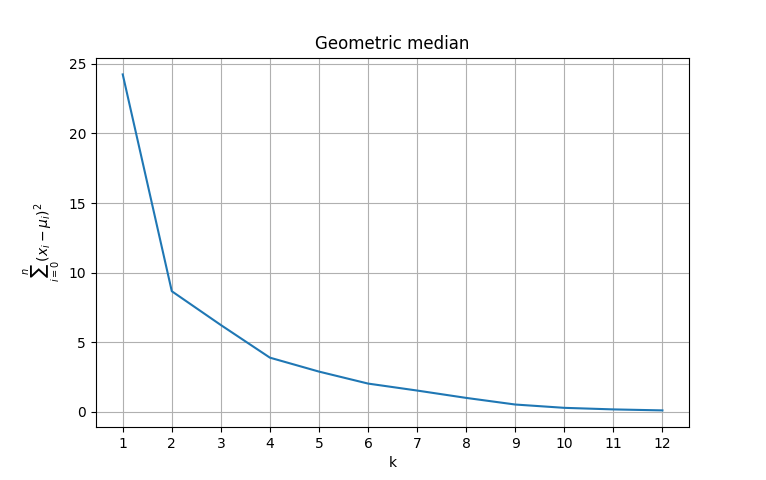
\includegraphics[width=.8\textwidth]{ex1_geometric_median}
    \end{center}
    \caption{Distance en fonction de \textit{K}}
    \label{Distance en fonction de \textit{K}}
\end{figure}

Nous graphique nous montre que nous trouvons des variations importantes pour $K\in\{2, 4\}$.
Après quelques tests empiriques nous avons fixé $K=4$.


\subsection{Affichage des données \textit{K}}

Les données normalisées et transformées sont affichés:

\begin{figure}[H]
    \begin{center}
        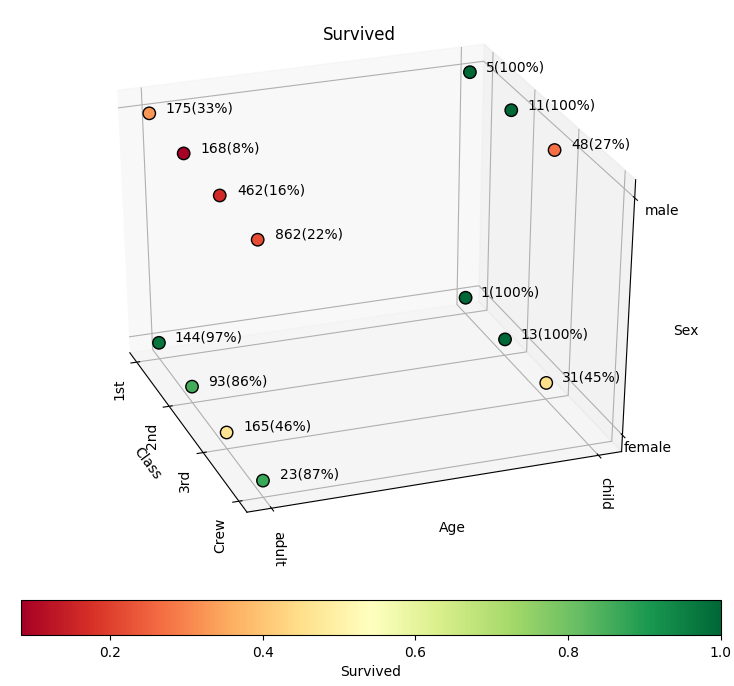
\includegraphics[width=.8\textwidth]{ex1_survived}
    \end{center}
    \caption{Survie selon paramètres}
    \label{Survie selon paramètres}
\end{figure}


Chaque point est accompagné de l'information du nombre de personnes ayant ces paramètres et le pourcentage de personnes ayant survécu.
L'échelle de couleur nous renseigne sur la quantité de personnes ayant survécu, allant du rouge pour 0\% jusqu'au vert pour 100\%.


\subsection{Clustering}

Voici le résultat du clustering:

\begin{figure}[H]
    \begin{center}
        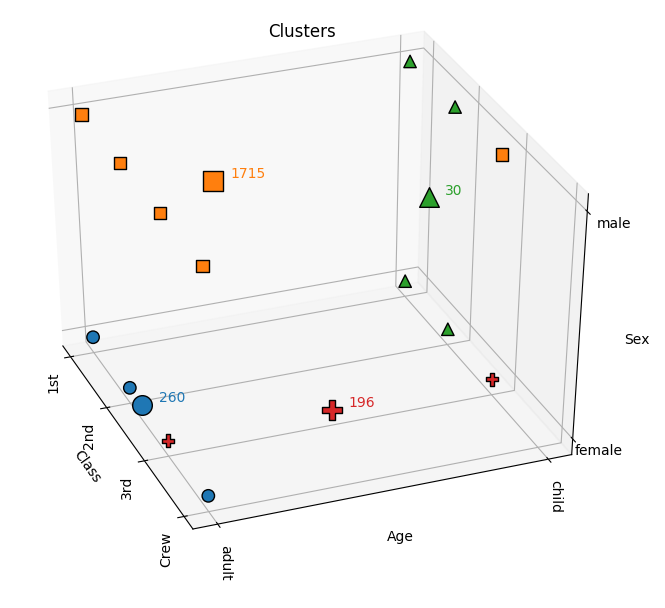
\includegraphics[width=.8\textwidth]{ex1_clusters}
    \end{center}
    \caption{Clustering}
    \label{Clustering}
\end{figure}


Chaque point est représenté par un symbole et une couleur selon le cluster auquel le point appartient.

Un point supplémentaire du même symbole et couleur,
mais de taille plus large symbolise le centre du cluster et a inscrit le nombre de personnes de ce cluster.

\subsection{Commentaires}

Le cluster Triangle Vert forme un groupe de personnes qui sont caractérisées par:
\begin{itemize}
    \item leur age: ce sont des enfants;
    \item leur classe: 1ème ou 2ème classe;
    \item leur taux de survie: 100\%.\\
\end{itemize}


Le cluster Croix Rouge forme un groupe de personnes qui sont caractérisées par:
\begin{itemize}
    \item leur sexe: ce sont des femmes;
    \item leur classe: 3ème classe;
    \item leur taux de survie: autour des 50\%.\\
\end{itemize}

Le cluster Cercle Bleu forme un groupe de personnes qui sont caractérisées par:
\begin{itemize}
    \item leur age: ce sont des adultes;
    \item leur sexe: ce sont des femmes;
    \item leur classe: toute sauf la 3ème;
    \item leur taux de survie: au dessus de 86\%.\\
\end{itemize}

Le cluster Carré Orange forme un groupe de personnes qui sont caractérisées par:
\begin{itemize}
    \item leur sexe: ce sont des hommes;
    \item leur age/classe: ce sont des adultes ou 3ème classe;
\end{itemize}

Nous pouvons faire quelques remarques:
\begin{itemize}
    \item les hommes adultes ont très peu survécu;
    \item ceux de 3ème classe ou eu une mortalité bien plus importante;
    \item les enfants ont été épargnés, sauf ceux de 3ème classe;
    \item les femmes ont une une mortalité relativement basse, sauf celles de 3ème classe;
\end{itemize}


\newpage

% -----------------------------------------------------------------------------
\section{Classification supervisée imposée}
\subsection{Introduction}
\label{part2}

Le but de cette deuxième partie est de trouver par \textit{validation croisée}
la meilleure méthode de classification sur les données suivantes:
\begin{itemize}
    \item cancer du sein\footnote{\url{https://archive.ics.uci.edu/ml/datasets/Breast+Cancer+Wisconsin+(Diagnostic)}};
    \item vins\footnote{\url{https://archive.ics.uci.edu/ml/datasets/Wine}}. \\
\end{itemize}

Les méthodes de classification supervisée sont imposées et les voici:
\begin{itemize}
    \item méthode des k-plus proches voisins;
    \item arbres de décision;
    \item perceptron multi-couche. \\
\end{itemize}

Pour la méthode des k-plus proches voisins, le paramètre \textit{K} est fait varier de 1 à 10 compris. \\
Pour la méthode des arbres de décision,
le nombre minimum d'échantillon dans une feuille est fait varier de 1 à 10 compris. \\
Concernant la méthode du Perceptron multi-couche,
toutes les combinaisons de solveurs et de fonctions d'activation possibles sont testées. \\

La validation croisée divise les données en 5 parties et est répétée 10 fois.
Cela implique qu'il y aura au total 50 scores de performance pour une méthode donnée.
Les résultats de cette validation croisée sont ensuite tracés sur un graphe,
permettant de comparer les performances des différentes méthodes. \\

Chaque graphe est tracée selon la légende suivante: \\
En abscisse, nous avons la variation de ou des paramètres intéressants pour la méthode concernée. \\
En ordonnée, nous avons plusieurs choses.
Chaque point représente un score.
Ces points sont regroupés par couleur, qui représente les variations de la méthode.
Les barres horizontales noires représentent la performance moyenne pour la variation de la méthode concernée.
La barre horizontale rouge représente la meilleure performance moyenne parmi toutes les variations d'une même méthode.

\newpage

% -----------------------------------------------------------------------------
\subsection{Données du cancer du sein}

Voici ci-dessous le résultat de la validation croisée pour les méthodes citées sur les données du cancer du sein:

\begin{figure}[H]
    \begin{center}
        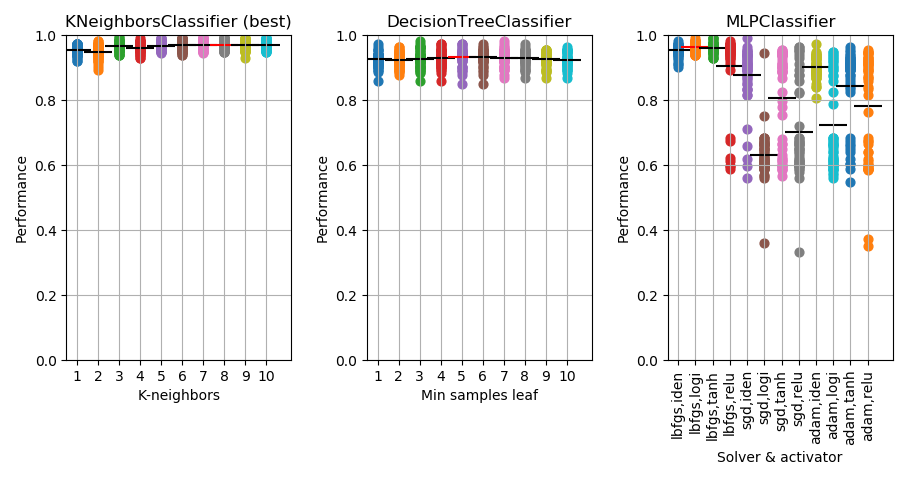
\includegraphics[width=1\textwidth]{ex2_breastcancer}
    \end{center}
    \caption{Résultat de la validation croisée sur les données du cancer du sein}
    \label{Résultat de la validation croisée sur les données du cancer du sein}
\end{figure}

De manière générale, les 3 méthodes, avec les paramètres adéquats, donnent des résultats satisfaisants.
En effet, la plupart des variations donne un score moyen qui dépasse les 90\%. \\

La méthode des k-plus proches voisins est ici pour peu la meilleure méthode.
La variation du paramètre \textit{K} n'affecte que de quelques pourcents le score moyen.
Par ailleurs, on peut observer qu'après $K = 6$,
le score moyen est stable et varie très peu. \\

Concernant la méthode des arbres de décision,
on remarque que la courbe construite à partir des scores moyens produit un pic lorsque
le nombre d'éléments minimums dans un nœud feuille est de 5.
On peut donc en déduire que les données peuvent facilement être regroupé par 5.
Ceci explique également le \textit{K} obtenu pour la méthode des k-plus proches voisins. \\

Quant au Perceptron multi-couche, les différents solveurs donnent des résultats bien différents,
alors que changer la fonction d'activation ne produit que peu d'effet,
excepté certaines combinaisons,
comme le solveur \textit{sdg (stochastic gradient descent)} et la fonction d'activation \textit{logistic (fonction sigmoid)} qui
produit un effet désastreux.
Cependant, cette même fonction d'activation marche très bien avec le solveur \textit{lbfgs} (\textit{Limited-memory Broyden–Fletcher–Goldfarb–Shanno}),
produisant un résultat similaire à la méthode des k-plus proches voisins.
Le solveur présentant les meilleurs résultats est le \textit{lbfgs}.

\newpage

% -----------------------------------------------------------------------------
\subsection{Données des vins}

Voici ci-dessous le résultat de la validation croisée pour les méthodes citées sur les données des vins:

\begin{figure}[H]
    \begin{center}
        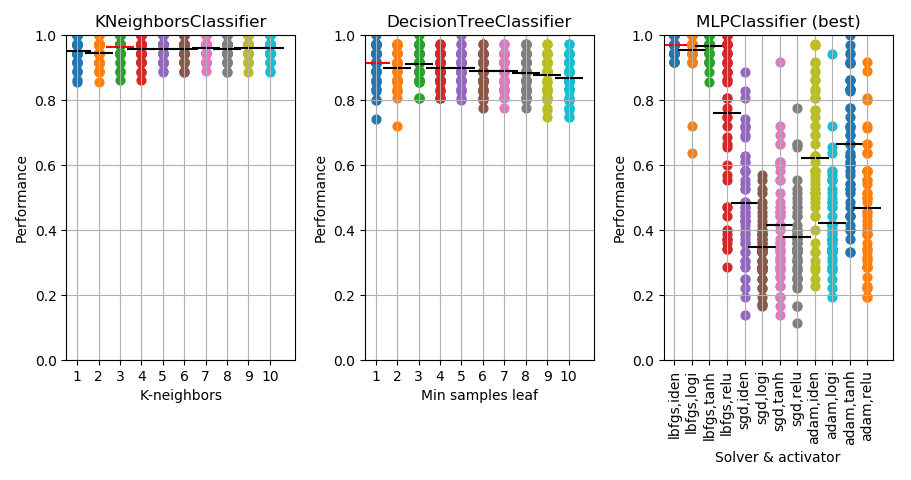
\includegraphics[width=1\textwidth]{ex2_wine}
    \end{center}
    \caption{Résultat de la validation croisée sur les données des vins}
    \label{Résultat de la validation croisée sur les données des vins}
\end{figure}

Par rapport au données du cancer du sein,
on remarque immédiatement que les scores sont de manière générale plus étalés.
On peut donc en déduire que ces données se regroupent moins facilement.
On peut par ailleurs bien l'observer avec la méthode des arbres de décision,
où l'on voit que la meilleure variation est lorsqu'il n'y a qu'un seul élément dans un nœud feuille. \\

Pour ces données, la meilleure méthode est le Perceptron multi-couche.
Nous retrouvons encore le solveur \textit{lbfgs},
mais cette fois avec la fonction d'activation \textit{identité} au lieu de la \textit{sigmoid}.
On voit également que les autres solveurs, quelque soit la fonction d'activation, sont mauvais avec ces données. \\

Pour peu, la méthode des k-plus proches voisins n'est pas la meilleure.
Ceci dit, toutes les variations de cette méthode sont bonnes.
Le paramètre \textit{K} n'a que peu d'effet.

\newpage

% -----------------------------------------------------------------------------
\section{Classification supervisée libre}

La partie 3 de ce travail suit le même principe que la partie 2 (voir section \ref{part2}),
mais les 3 méthodes ainsi que les données sont à choix. \\

Les données choisies sont celles caractérisant les feuilles de plantes\footnote{\url{https://archive.ics.uci.edu/ml/datasets/Leaf}}.
Chaque feuille est accompagnée du nom de l'espèce auquelle elle appartient, représentant ici la classe recherchée. \\

Les 3 méthodes choisies sont les suivantes:
\begin{itemize}
    \item support vector machines;
    \item forêts aléatoires;
    \item arbres de décision. \\
\end{itemize}

Pour la méthode des support vector machines, tous les noyaux sont testés. \\
Pour la méthode des forêts aléatoires ainsi que celle des arbres de décision,
le nombre minimum d'échantillon dans une feuille est fait varier de 1 à 10 compris. \\

Voici ci-dessous le résultat de la validation croisée pour les méthodes citées sur les données choisies:

\begin{figure}[H]
    \begin{center}
        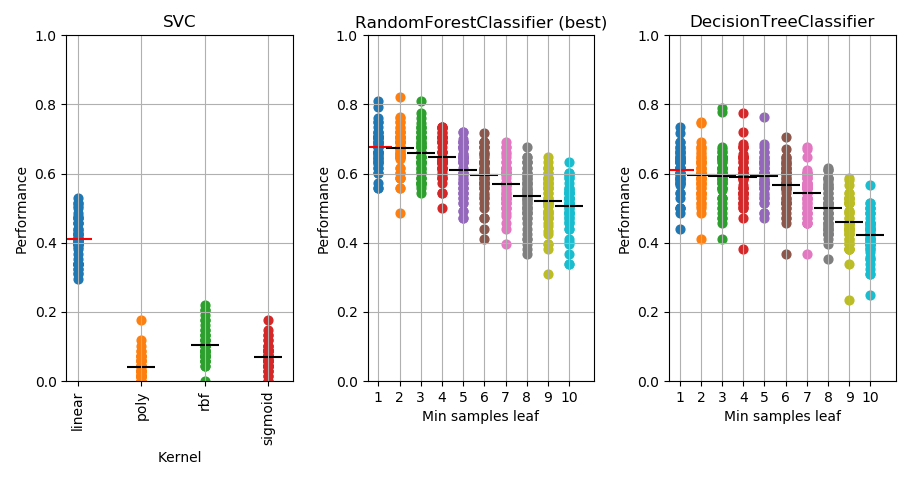
\includegraphics[width=1\textwidth]{ex3}
    \end{center}
    \caption{Résultat de la validation croisée sur les données des feuilles de plantes}
    \label{Résultat de la validation croisée sur les données des feuilles de plantes}
\end{figure}

La première méthode, le SVC, est simplement mauvaise, quelque soit le noyau choisi.
Le noyau \textit{linéaire} est le seul à donner un résultat décent.
Ceci dit, les paramètres ont tous été laissés par défaut. \\

La meilleure méthode est celle des forêts aléatoires.
On remarque que de forcer plus d'un élément dans une feuille ne fait qu'empirer le score.
On peut en déduire que les données ne peuvent être regroupées facilement. \\

La méthode des arbres de décision a ici été utilisée pour comparer ses performances à la méthode des forêts aléatoires.
On remarque le même effet concernant le nombre d'éléments minimums.
De manière générale, cette méthode produit un score un peu inférieur à la méthode des forêts aléatoires.

\newpage

% -----------------------------------------------------------------------------
\section{Conclusion}

\end{document}
